72. $$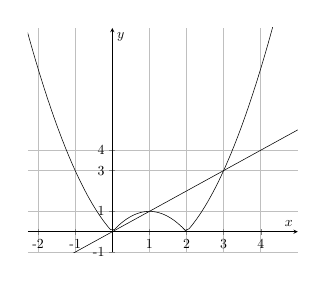
\begin{tikzpicture}[scale=0.5]
\begin{axis}[
    axis lines = middle,
    grid=major,
    legend pos={south west},
    xlabel = {$x$},
    %xlabel style={below right},
    ylabel = {$y$},
    ymin=-1,
    ymax=10,
    xtick={-2,-1,1,2, 3, 4},
    xticklabels={-2,-1,1,2, 3, 4},
    ytick={-2,-1,1, 3, 4},
    yticklabels={-2,-1,1, 3, 4},
                  ]
	\addplot[domain=-5:5, samples=100, color=black] {abs(x*x-2*x)};
    %\addplot[domain=-0.99:0.5, samples=100, color=black] {1/(1-x)};
    \addplot[domain=-5:5, samples=100, color=black] {x};
   % \addplot[domain=1.01:5, samples=100, color=black] {3/(x+1)};
    %\addlegendentry{$\text{Рис. 1}$};
\end{axis}
%\draw (2.75,2.82) circle (2pt);
%\draw (4.11,3.98) circle (2pt);
\end{tikzpicture}$$
 По графику найдём ответ $x \in [1;3]\cup\{0\}.$\\
